\newpage
\section{Fundamentos Teóricos}
Filtros passa-faixa e rejeita-faixa são circuitos RLC com frequência variável, que conseguem selecionar para sua saída determinados um intervalo de sinais de entrada, atenuando ou acentuando sinais que estejam fora da faixa de passagem. É fato que a resposta de um circuito é dependente de suas impedâncias, logo, uma vez que a impedância é uma função da frequência, tem-se que esta é a principal distinção entre um circuito com frequência constante e outro com frequência variável.

No estudo de resposta em frequência, tem-se que a amplitude e a fase da saída variam somente se a amplitude e a fase da função de transferência também variam, à medida que a frequência é alterada. A função de transferência no circuito de filtro utilizado neste experimento, cujos possuem tensões senoidais como entrada e saída, é dada pela razão entre a tensão de saída e a tensão de entrada.

\begin{figure}[ht]
	\centering
	\caption{Circuito RLC com entrada e saída de tensão, no domínio da frequência .}
	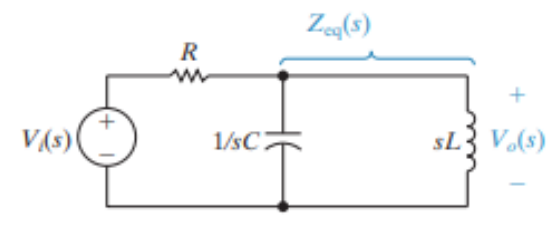
\includegraphics[width=10cm]{images/circuitotensao.png}
	\caption*{Fonte:\cite{nilsson2008circuitos}.}
	\label{circuito}
\end{figure}

\begin {equation}
H(s) = \frac{V_o(s)}{V_i(s)}
\label{transferencia}
\end {equation}

O que diferencia um circuito filtro passa-faixa para filtro rejeita-faixa é a análise de seu gráfico de resposta. Os gráficos, mostrados adiante, ilustram a variação da função de transferência com a variação da fonte, onde tem-se os valores de $|H(j\omega)|$ em função da frequência $\omega$ sendo o gráfico da amplitude, e $\theta(j\omega)$ em função da frequência $\omega$ sendo o gráfico de fase.

\subsection{Filtro passa-faixa}

Os filtros passa-faixa são nomeados dessa forma devido ao gráfico de resposta, onde nota-se que o circuito permite apenas a saída de um intervalo entre as frequências de corte $\omega_{c1}$ e $\omega_{c2}$, de modo que atenue as frequências fora desse intervalo, sendo a largura de faixa de passagem, denominada de $\beta$, indicado na equação \ref{beta}, em $rad/s$. A tensão de saída para esse filtro é dada sob os terminais do indutor.

\begin{equation}
	\beta = \omega_{c2} - \omega_{c2} = \frac{1}{RC} \qquad [rad/s]
	\label{beta}
\end{equation}

\begin{figure}[ht]
	\centering
	\caption{Gráfico do filtro passa-faixa ideal.}
	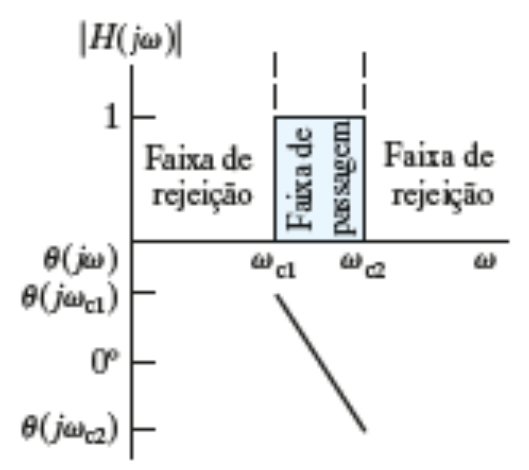
\includegraphics[width=6cm]{images/graficoPassaFaixaIdeal.png}
	\caption*{Fonte:\cite{nilsson2008circuitos}.}
	\label{graficoPassaFaixaIdeal}
\end{figure}

\begin{figure}[ht]
	\centering
	\caption{Gráfico do filtro passa-faixa.}
	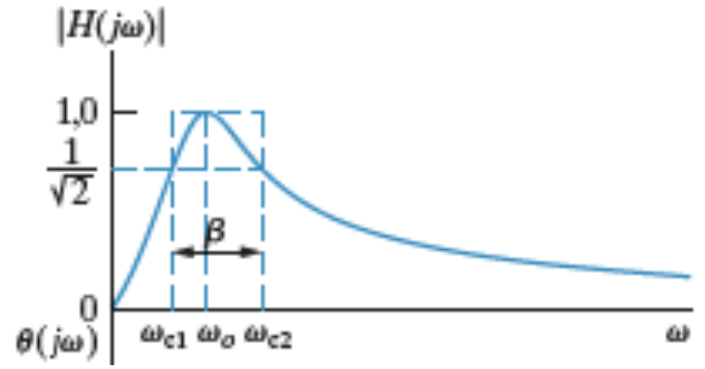
\includegraphics[width=10cm]{images/graficoFiltroPassaFaixa.png}
	\caption*{Fonte:\cite{nilsson2008circuitos}.}
\end{figure}

Alguns parâmetros são importantes para a análise dos filtros. A frequência de ressonância, ou natural, $\omega_0$, definida quando quando a função de transferência é um real puro, ou seja, sem parte imaginária; é o valor de frequência que correspondente ao máximo valor do módulo da . Pode ser matematicamente definido pelas equações \refeq{frequência de ressonância 1} ou
\refeq{frequência de ressonância 2}.

\begin {equation}
\omega_0 = \sqrt{\frac{1}{L C}} \qquad [rad/s]
\label{frequência de ressonância 1}
\end {equation}

\begin {equation}
\omega_0 = \sqrt{ {\omega_{c1}}^2 {\omega_{c2}}^2 } \qquad [rad/s]
\label{frequência de ressonância 2}
\end {equation}

O fator de qualidade $Q$, é a medida da largura da faixa de passagem, independente da da localização no eixo das frequência $\omega$.

\begin {equation}
Q = \frac{\omega_0}{\beta}
\label{fator de qualidade}
\end {equation}

Realizando uma análise qualitativa do circuito apresentado na Figura \ref{circuito}, observamos que: Quando $\omega = 0$, o capacitor pode ser considerado um circuito aberto e o indutor um curto-circuito, logo a tensão $V_o(s) = 0 V$. E quando $\omega \rightarrow \infty $, a situação inverte, o capacitor é curto-circuito e o indutor um circuito aberto, então $V_o(s) = 0 V$ dá mesma forma. Já na frequência de ressonância, formulada nas equações \ref{frequência de ressonância 1} e \ref{frequência de ressonância 2}, a impedância combinada tende ao infinito, logo $V_o(s) = V_i(s)$.
Então, nos valores entre as frequências de corte a amplitude da tensão de saída será diferente tensão de entrada, porem não nula.

A função de transferência do circuito $H(s)$ , considerando o indutor como tensão de saída, pode ser obtida primeiramente calculando a impedância equivalente do circuito. Notamos que o sistema é um divisor de tensão, logo:

\begin {equation}
Z_{eq} = \frac{ \frac{L}{C} }{ sL + \frac{1}{sC}}
\end {equation}

Sendo assim, a tensão de saída $V_o (s)$ é dada por:

\begin {equation}
V_o (s) = \frac{Z_{eq}}{Z_{eq} + R} V_i(s) = \frac{\frac{s}{RC}}{ s^2 + \frac{s}{RC} + \frac{1}{LC} } V_i(s) \qquad [V]
\label{V0 passa-faixa}
\end {equation}

Substituindo a equação \refeq{V0 passa-faixa} em \refeq{transferencia}, obtemos:

\begin {equation}
H(s) = \frac{ \frac{s}{RC} }{ s^2 + \frac{s}{RC} + \frac{1}{LC} }
\end {equation}

Se $s=j\omega$, então:

\begin {equation}
H(j \omega) = \frac{\frac{j \omega}{RC}}{ (j \omega)^2 + \frac{j \omega}{RC} + \frac{1}{LC} }
\end {equation}

O módulo de um número complexo é dado pela raiz quadrada da soma dos quadrados do número imaginário e real. Portanto, o módulo dado pela função de transferência é dado por:

\begin {equation}
|H(j \omega)| = \frac{ \frac{\omega}{RC} }{ \sqrt{  ( \frac{ 1 }{LC} - \omega^2 )^2 + (\frac{\omega}{RC})^2} }
\label{moduloFuncaoTransferencia}
\end {equation}

Quando $|H(j \omega)|$ é máximo, temos a que $\omega$ é a frequências natural, onde a primeira parte da soma, dentro da raiz da equação \ref{moduloFuncaoTransferencia} é nula. Isso nos leva a equação \ref{frequência de ressonância 1}.

Já para as frequências de corte $\omega_{c1}$ e $\omega_{c2}$ temos a equação \ref{frequencia de corte}. Como o valor $H_{max} = 1$ para os filtros passivos (passa-altas, passa-baixas, passa-faixa e rejeita-faixa), então ela é constante. Vale ressaltar que a diferença entre filtros ativos e passivos se dá pelos componentes presentes no sistema, se eles forem passivos (capacitores, indutores e resistores) e o filtro também é passivo, já se forem ativos (amplificador
operacional, por exemplo), o filtro é classificado como ativo.

\begin{equation}
	|H(j \omega_{cn})| = \frac{1}{\sqrt{2}} H_{max} = \frac{1}{\sqrt{2}}
	\label{frequencia de corte}
\end{equation}

Substituindo a equação \ref{frequencia de corte} na equação \ref{moduloFuncaoTransferencia}, obtemos o equacionamento de ambas as frequências de corte em $rad/s$:

\begin{equation}
	\omega_{c1} = - \frac{1}{2RC} + \sqrt{ (\frac{1}{2RC})^2 + \frac{1}{LC} } \qquad [rad/s]
	\label{omegaC1}
\end{equation}

\begin{equation}
	\omega_{c2} = + \frac{1}{2RC} + \sqrt{ (\frac{1}{2RC})^2 + \frac{1}{LC} } \qquad [rad/s]
	\label{omegaC2}
\end{equation}

\pagebreak

\subsection{Filtro rejeita-faixa}

Ao contrário do passa faixa, esse filtro permite a passagem de qualquer frequência que não esteja no intervalo entre as frequências de corte $\omega_{c1}$ e $\omega_{c2}$, e atenua valores nesse intervalo, como apresentado na Figura \ref{graficoRejeitaFaixaIdeal}. A tensão de saída para esse filtro é dada sob os terminais do resistor.

\begin{figure}[ht]
	\centering
	\caption{Gráfico do filtro rejeita-faixa ideal.}
	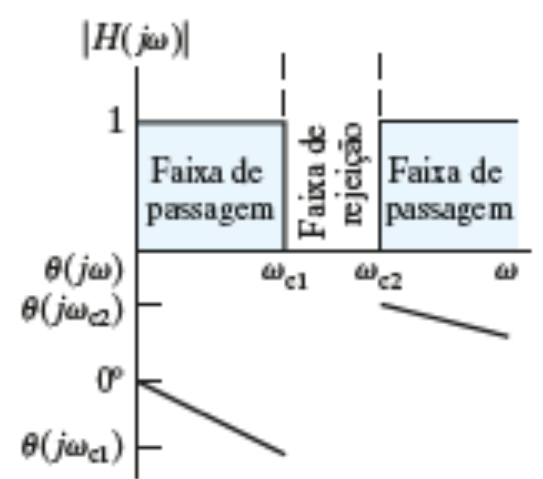
\includegraphics[width=6cm]{images/graficoRejeitaFaixaIdeal.png}
	\caption*{Fonte:\cite{nilsson2008circuitos}.}
	\label{graficoRejeitaFaixaIdeal}
\end{figure}

\begin{figure}[ht]
	\centering
	\caption{Gráfico do filtro rejeita-faixa.}
	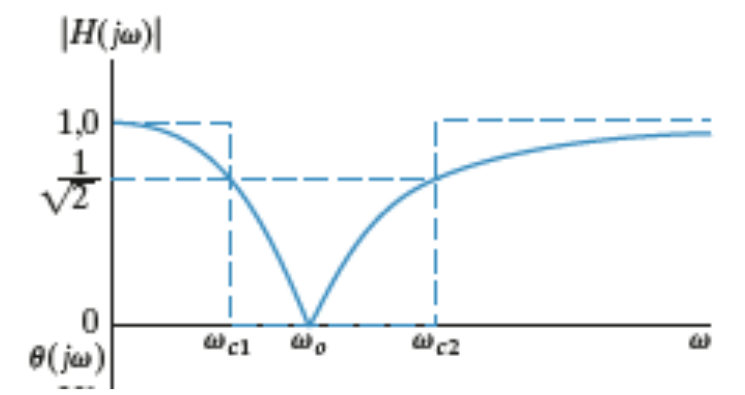
\includegraphics[width=9cm]{images/graficoFiltroRejeitaFaixa.png}
	\caption*{Fonte:\cite{nilsson2008circuitos}.}
\end{figure}

A frequência natural $\omega_0$, de um rejeita-faixa é o valor de frequência que correspondente ao mínimo, ou seja, nulo da função de transferência. Os parâmetros, definidos pelas equações \ref{beta}, \ref{frequência de ressonância 1}, \ref{frequência de ressonância 2} e \ref{fator de qualidade}, podem ser aplicadas em ambos os filtros.

Para a analíse qualitativa, vale lembrar que os estados de dos bipolos para $\omega = 0$ e $\omega \rightarrow \infty $ é o mesmo, já que trata-se do mesmo circuito, só mudando o sinal de saída. Quando $\omega = 0$ ou $\omega \rightarrow \infty $, $V_o(s) = V_i(s)$.

Para encontrarmos a função de transferência do filtro rejeita-faixa primeiro devemos observar que, pela analíse de malha obtemos as seguintes relações:

\begin{equation}
	V_i(s) = I (\frac{sL}{s^2LC+1}+R) \qquad [V]
\end{equation}

\begin{equation}
	V_o(s) = IR \qquad [V]
\end{equation}

A partir disso, seguimos os mesmos passos discutidos no tópico anterior, então a função de transferência será:

\begin{equation}
	H(s) = \frac{s^2 + \frac{1}{LC}}{s^2 + \frac{s}{RC} + \frac{1}{LC}}
	\label{funcao tranferenci rejeita-faixa}
\end{equation}

Como $s=j\omega$:

\begin{equation}
	H(j\omega) = \frac{-\omega^2 + \frac{1}{LC}}{-\omega^2 + \frac{j\omega}{RC} + \frac{1}{LC}}
	\label{funcao tranferenci rejeita-faixa jw}
\end{equation}

Calculando o módulo da função:

\begin {equation}
|H(j \omega)| = \frac{ (\frac{1}{LC})^2 - \omega^2 }{ \sqrt{  ( \frac{ 1 }{LC} - \omega^2 )^2 + (\frac{\omega}{RC})^2} }
\label{moduloFuncaoTransferencia2}
\end {equation}

Por fim, ao analisarmos a equação \ref{moduloFuncaoTransferencia2}, da mesma forma do tópico anterior, obteremos as mesmas equações \refeq{omegaC1} e \refeq{omegaC2}.

\pagebreak
